% Adjust these for the path of the theme and its graphics, relative to this file
%\usepackage{beamerthemeFalmouthGamesAcademy}
\usepackage{../../beamerthemeFalmouthGamesAcademy}
\usepackage{multimedia}
\graphicspath{ {../../} }

% Default language for code listings
\lstset{language=C++,
        morekeywords={each,in,nullptr}
}

% For strikethrough effect
\usepackage[normalem]{ulem}
\usepackage{wasysym}
\usepackage{gensymb}
\usepackage{pdfpages}

% http://www.texample.net/tikz/examples/state-machine/
\usetikzlibrary{arrows,automata}

\newcommand{\modulecode}{COMP260}\newcommand{\moduletitle}{Distributed Systems}\newcommand{\sessionnumber}{5}

\begin{document}
\title{\sessionnumber: Session title here}
\subtitle{\modulecode: \moduletitle}

\frame{\titlepage} 


\begin{frame}
	\frametitle{Immersion}
	Immersion is the objective degree to which a VR system and application projects stimuli onto the sensory receptors. We discuss immersion in terms of:

	\begin{itemize}
		\item Extensiven - Range of sensory modalities targeted 
		\item Matching - Stimuli vs reality
		\item Surrounding - Extent of environment (panoramic) and tracking
		\item Vividness - The quality of simulation
		\item Intractability - The quality of the input and outputs
		\item Plot - How compelling the narrative is
	\end{itemize}
\end{frame}

\begin{frame}
	\begin{figure}
		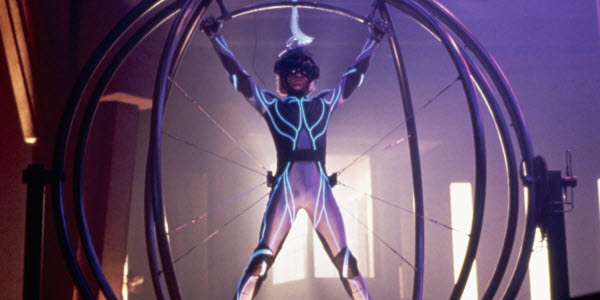
\includegraphics[scale=.6]{assets/mower} 
		\caption{The Lawnmower Man - 1992}
	\end{figure}
\end{frame}


\begin{frame}
	\frametitle{Immersion vs. Presence}
	
	`Presence is the psychological state of subjective perception in which even though part or all of an individual's current experience is generated by and/or filtered through human-made technology, part or all of the individual's perception fails to accurately acknowledge the role of the technology in the experience.' \\~\\
	
	International Society for Presence Research, 2000
	\\~\\
	\href{http://ispr.info}{[ISPR Website]}	
	
\end{frame}

\begin{frame}
	\frametitle{Next Week}
	We will cover presence through the psychological state of subjective perception and illusions that help facilitate VR sytems.
\end{frame}

\begin{frame}
	\frametitle{Perceptual Modalities}
	
	``A perceptual modality can be defined as the means through which information is extracted from the environment'' (James and Galbraith, 1985) \\~\\
	
	Immersion is created by surrounding the user of the VR system in images, sound or other stimuli that provide an engrossing total environment. \\~\\
	In order to achieve an illusion of immersion a reality system must consider the perceptual modalities: \textbf{Sight}, \textbf{hearing}, touch, proprioception, balance/motion, smell and taste. \\~\\
	
\end{frame}

\begin{frame}
	\begin{center}
		\href{https://www.youtube.com/watch?v=gvozcv8pS3c}{ 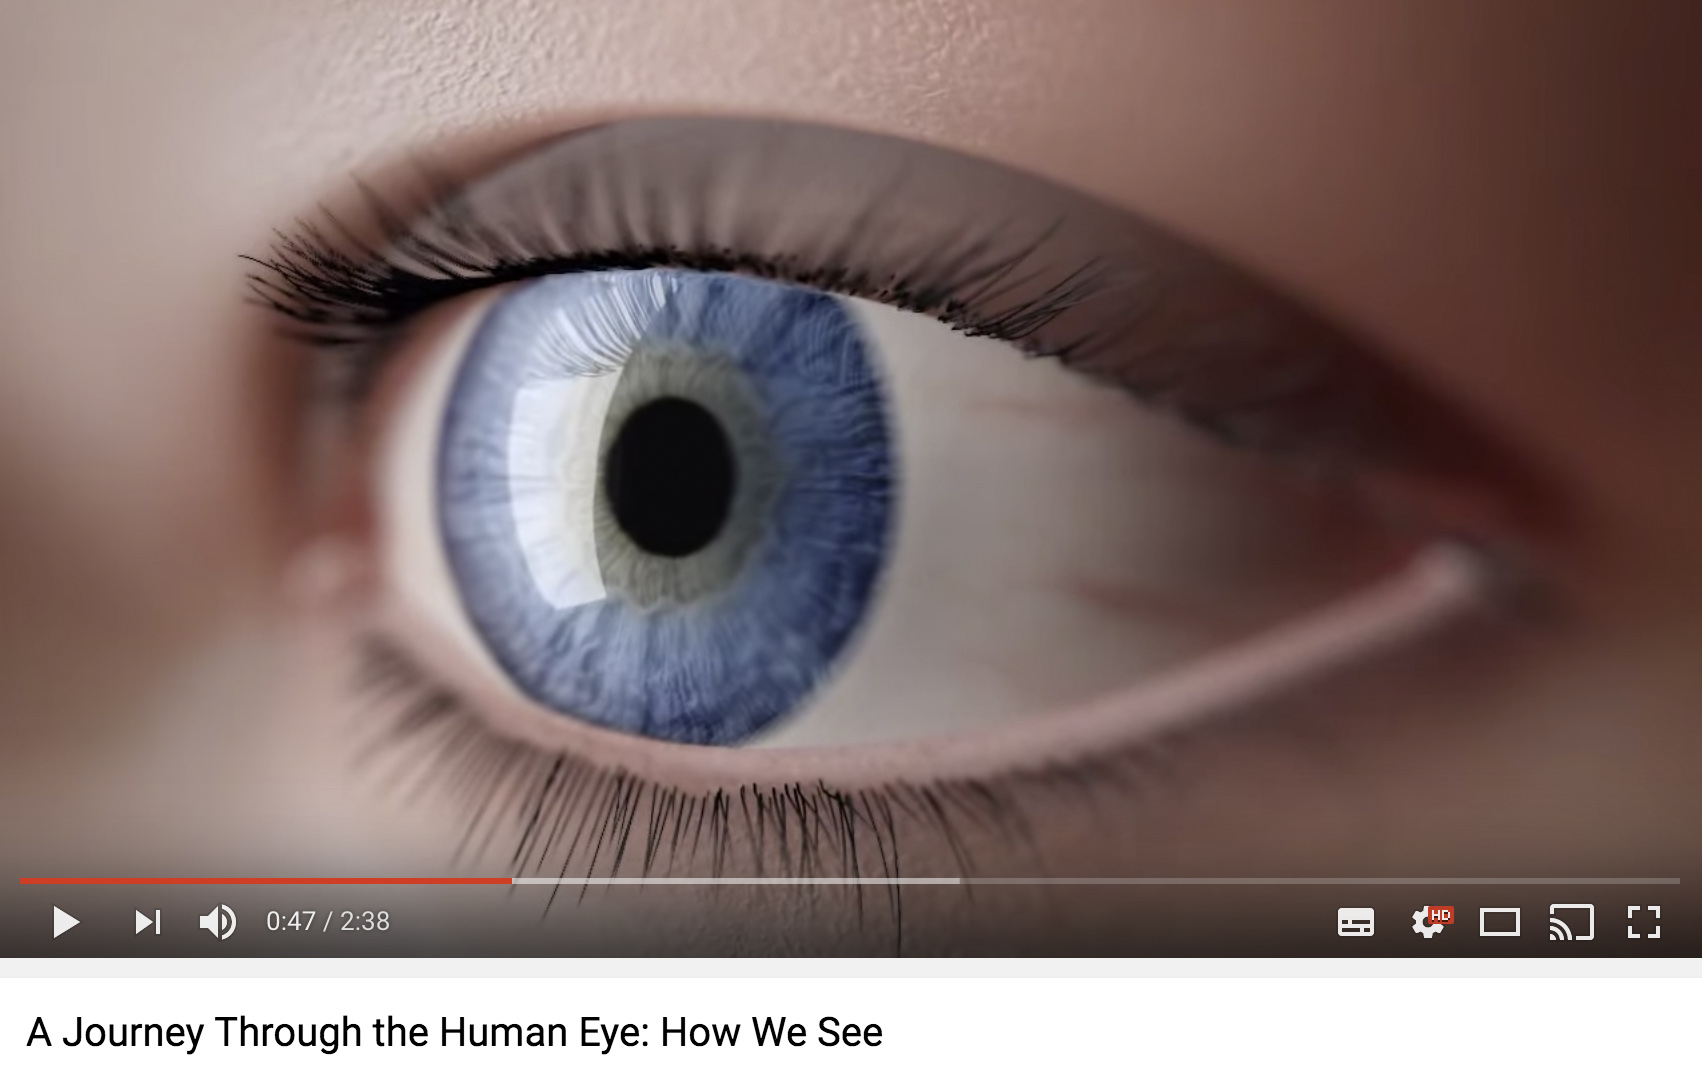
\includegraphics[scale=.3]{assets/eyetut}  }
	\end{center}
\end{frame}

\begin{frame}
	\begin{figure}
		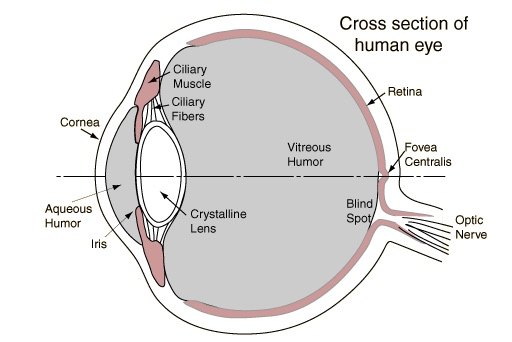
\includegraphics[scale=.6]{assets/eye} 
		\caption{}
	\end{figure}
\end{frame}

\begin{frame}
	\frametitle{Cones and Rods}
	\begin{figure}
		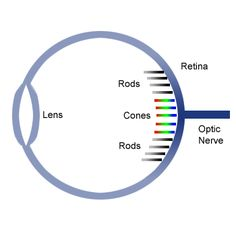
\includegraphics[scale=.5]{assets/cones-rods.jpg}
		\caption{ The retina is covered in two types of photoreceptors, cones and rods. Cones are responsible for vision in ideal conditions and rods are responsible for low light levels and non-ideal conditions. }
	\end{figure}
\end{frame}


\begin{frame}
	\frametitle{Central vs. Peripheral Vision}
	\textbf{Central}
	\begin{itemize}
		\item has high visual acuity,
		\item optimised for bright daytime conditions, and
		\item is color sensitive.
	\end{itemize}
	
	\textbf{Peripheral Vision}
	\begin{itemize}
		\item is color insensitive, 
		\item is more sensitive to light than central vision in dark conditions,
		\item is less sensitive to longer wavelengths (i.e., red),
		\item has faster response and has more sensitive to fast motion and flicker, and
		\item is less sensitive to slow motions.
	\end{itemize}
\end{frame}

\begin{frame}
	\frametitle{Field of View and Field of Regard}
	%The \textbf{field of view} is the angular measure of what can be seen at a single point in time. 
	\begin{figure}
		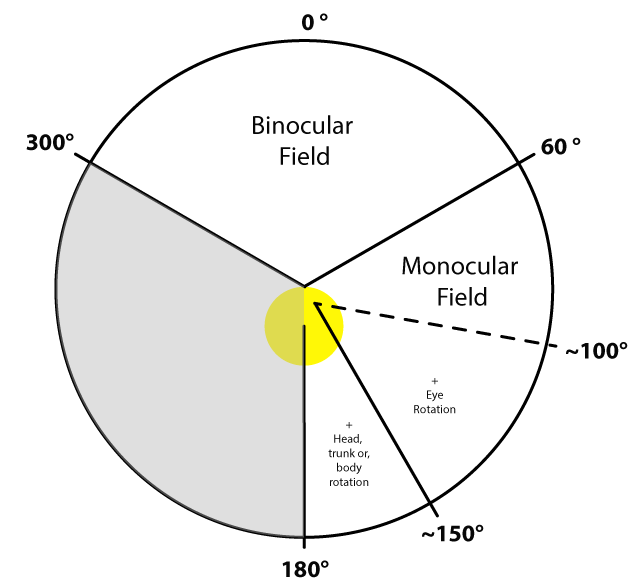
\includegraphics[scale=.3]{assets/fov} 
		\caption{Horizontal field of view of the right eye with straight ahead fixation (looking towards the top of the diagram)}
	\end{figure}
\end{frame}


%\begin{frame}
%	\frametitle{Visual Pathways}
%\end{frame}

\begin{frame}
	\frametitle{Arc Seconds \& Minutes}
	\pause
	\begin{figure}
		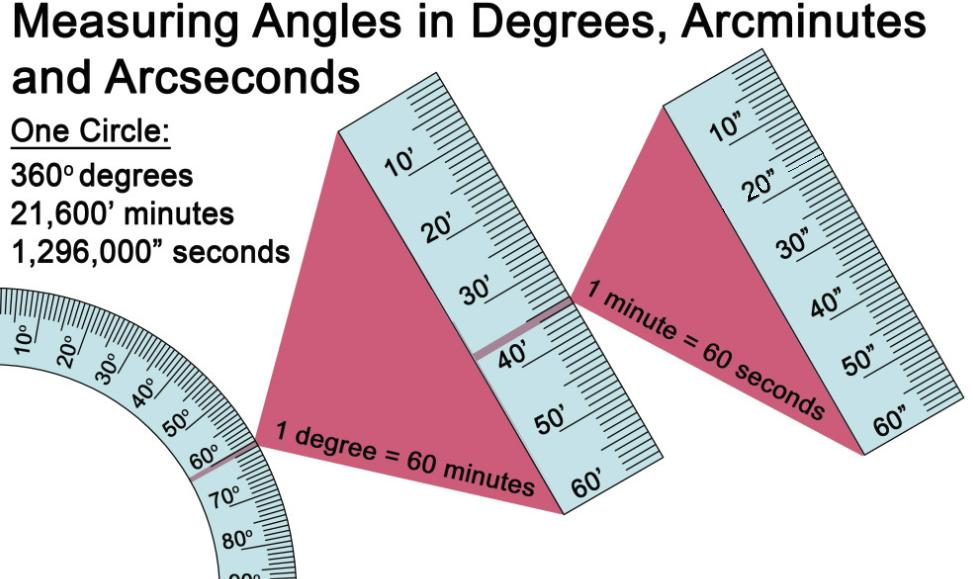
\includegraphics[scale=.4]{assets/arc} 
	\end{figure}
\end{frame}

\begin{frame}
	\frametitle{Acuity}
	Visual Acuity is the ability to resolve details and often measured in visual angle. \\~\\ \pause
	
	A fifty pence coin held at arms length has an angle of acuity of 2\degree \\~\\ \pause
	
	A fifty pence coin held up at 81 meters away has an angle of acuity of one arc min(1/60th of a degree). \\~\\ \pause
	
	In perfect conditions a human can see a line as thin as 0.5 are sec(1/7200th of a degree). 
\end{frame}

\begin{frame}
	\begin{figure}
		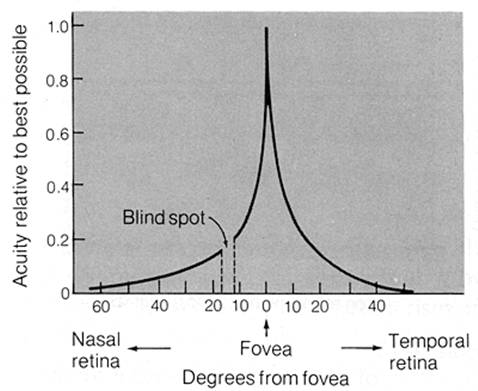
\includegraphics[scale=.9]{assets/acuity} 
		\caption{Visual acuity is much better at the fovea.}
	\end{figure}
\end{frame}

\begin{frame}
	The evidence suggests that given stereoscopic vision with each eye able to see 210\degree (including rotation) a display would need horizontal vision of 378,000 pixels for each eye to match what we see in reality. \\~\\
	\[ 210 * 60 * (60/2) = 378,000 \] \\~\\
	
	Obviously, this is an extreme analysis and there are ways that we can work around these limitations. 
\end{frame}

\begin{frame}
	\frametitle{VR Lenses}
	\begin{center}
		\href{https://www.youtube.com/watch?v=NCBEYaC876A}{ 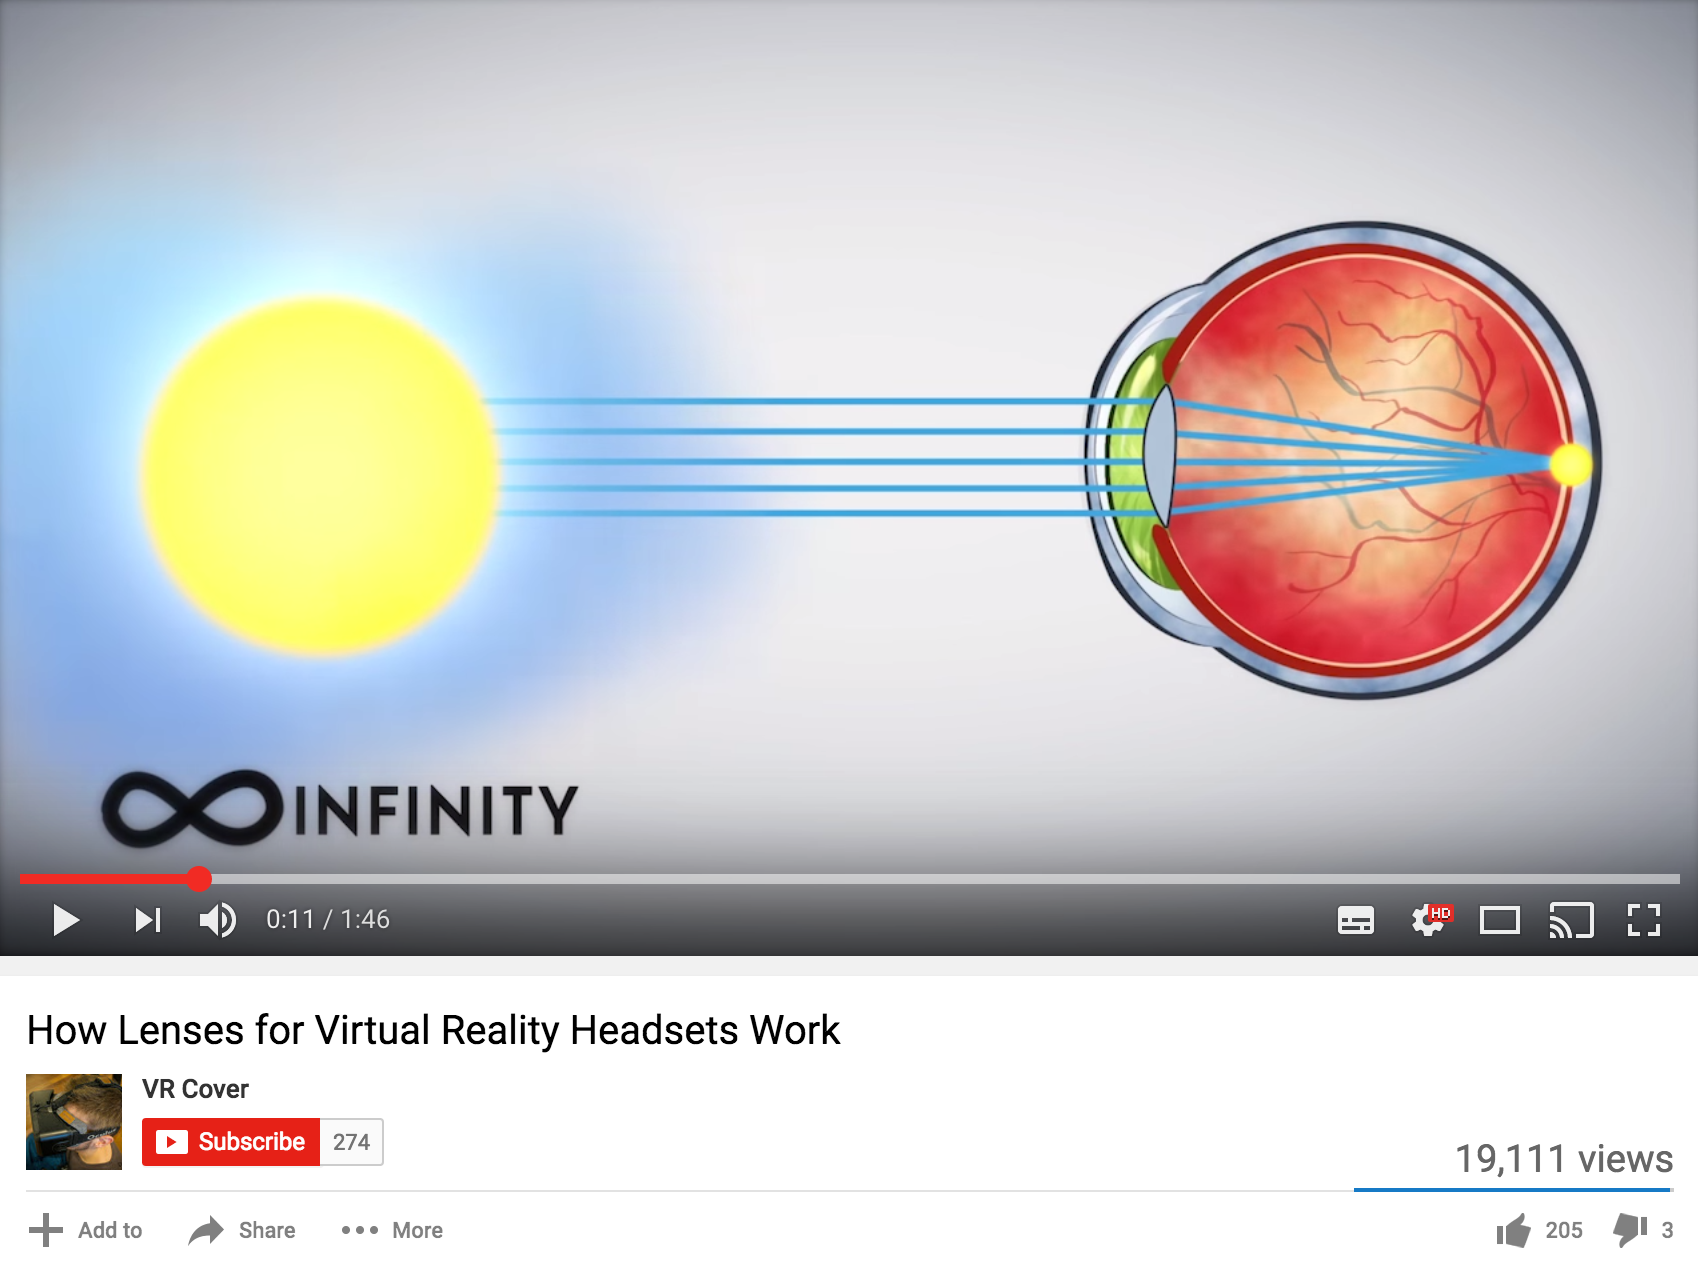
\includegraphics[scale=.3]{assets/lenses}  }
	\end{center}
\end{frame}

\begin{frame}
	\frametitle{Foveated Rendering}
	\begin{center}
		\href{https://www.youtube.com/watch?v=6q3w0fiD0zg}{ 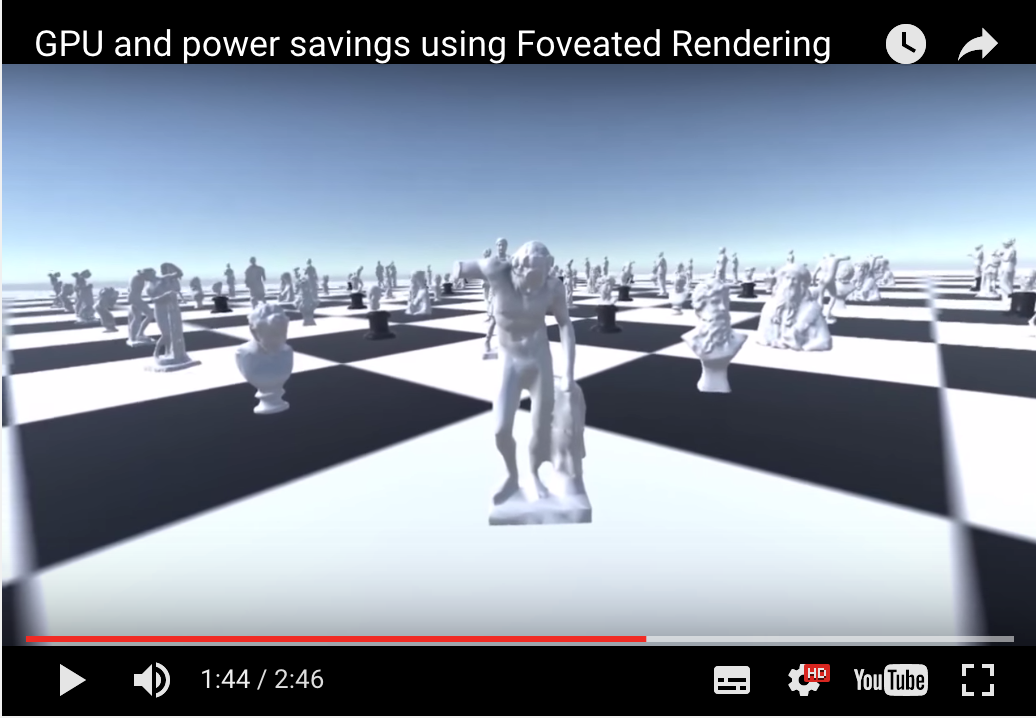
\includegraphics[scale=.4]{assets/foveated-rendering}  }
	\end{center}
\end{frame}

\begin{frame}
	\frametitle{Chromatic Aberration }
	
	\begin{figure}
		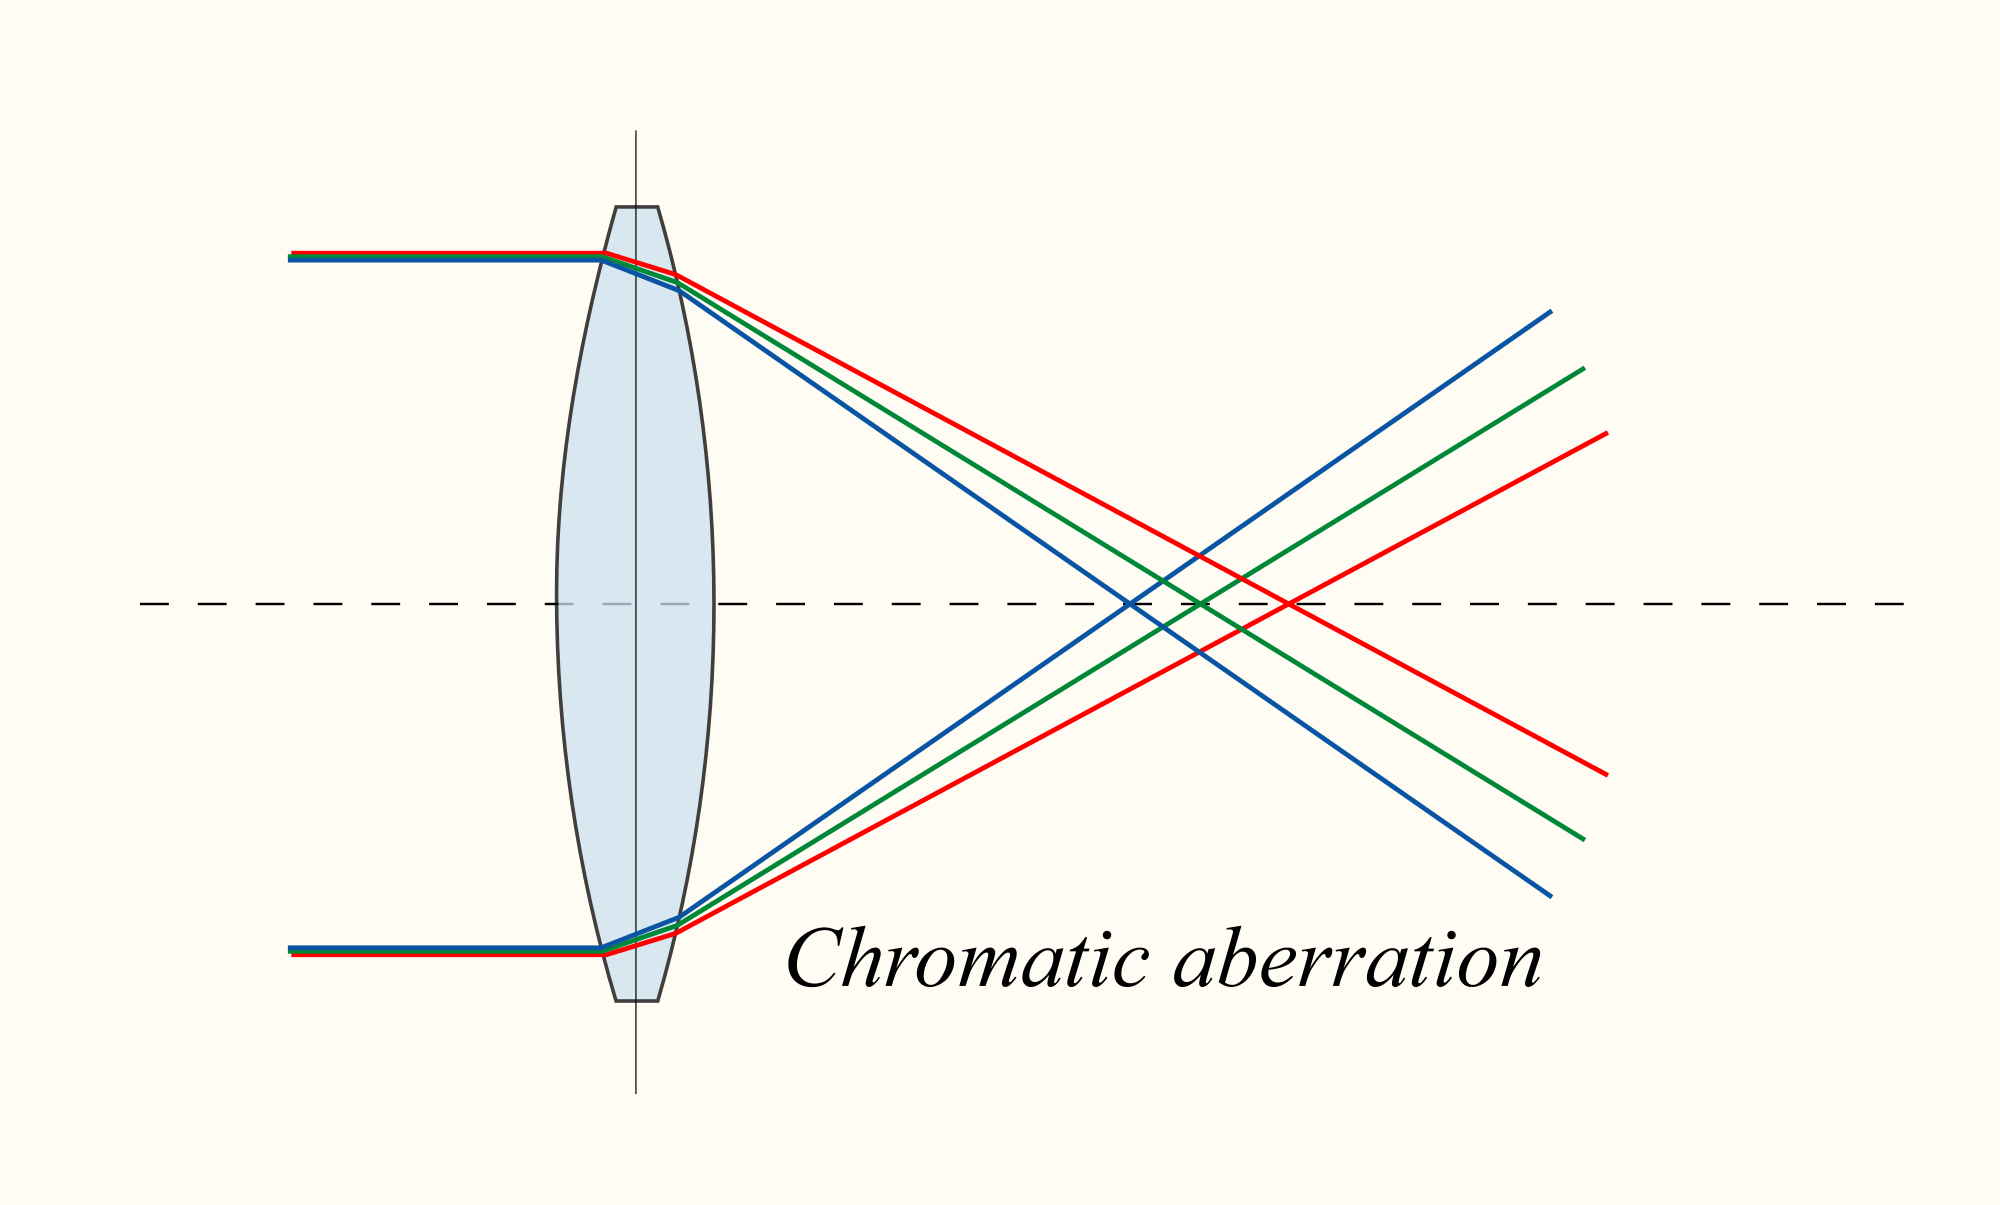
\includegraphics[scale=.1]{assets/aberration} 
		\caption{When different wavelengths of light refract at different angles. Movement of the eye can amplify the aberration. \tiny{aberration:a departure from what is normal}}
	\end{figure}
\end{frame}

\begin{frame}
	\frametitle{Vergence-Accommodation Conflict}
	
	\textbf{Vergence} - How your eyes track an object coming towards you. \\~\\

	\textbf{Accommodation} - When you pupils adjust to the objects light field. \\~\\
	
	The two actions are hardwired to work in sync as they are both trying aid the same process of tracking an object. They can be decoupled but it is not a comfortable experience for the user.

\end{frame}

\begin{frame}
	`After long session, I still have an hangover time though, as if I was on drugs the whole time and I need to readjust to reality.' \\~\\
	
	\href{https://www.reddit.com/r/oculus/comments/2clksh/question_for_dk2_owners_how_long_can_you_wear_it/cjgo683}{[link to further discussion]} \\~\\
	\href{https://www.reddit.com/r/oculus/comments/2epu1h/my_body_has_developed_a_fear_of_vr/}{and more}
	
\end{frame}

\begin{frame}
	\begin{figure}
		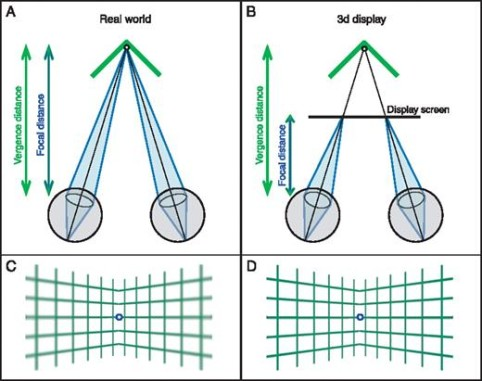
\includegraphics[scale=.7]{assets/verg} 
		\caption{Vergence-Accommodation Conflict}
	\end{figure}

\end{frame}

\begin{frame}
	\frametitle{Possible Solution}
	\begin{center}
		\href{https://www.youtube.com/watch?v=YJdMPUF8cDM}{ 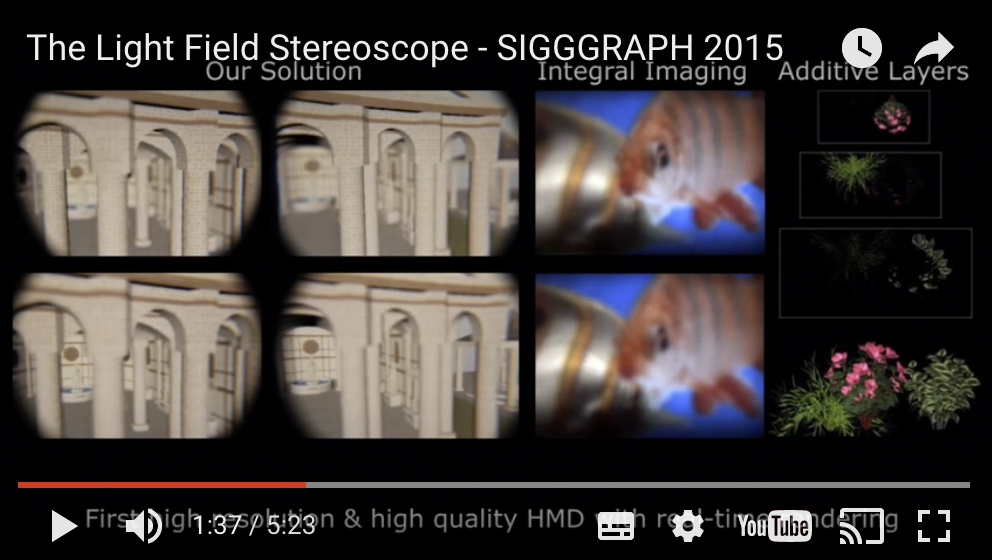
\includegraphics[scale=.55]{assets/lightfield}  }
	\end{center}

\end{frame}

\begin{frame}
	\frametitle{Motion to Photon Latency}
	\begin{itemize}
		\item \textbf{Motion} - refers to the users movements in the physical space.
		\item \textbf{Photons} - The photons emitted from the HMD that are absorbed by photoreceptors (cones \& rods) on the retina.
		\item \textbf{Latency} - delay between the two. 
	\end{itemize}
	
		Put simply, motion to photon latency is the time it takes for the users movements in physical space to be visualised on the head-mounted display(HMD).
	
\end{frame}

\begin{frame}
	\frametitle{Side Effects}
	The \textless20ms motion-to-photon latency gold standard. \\~\\
	
	When the motion to photon latency is greater than 20ms or anytime there is inconsistent stimuli between the players physical body motions and the visuals displayed in the head-mounted display (HMD) then there is a good chance that motion sickness/simulator sickness will occur. \\~\\

	According to the Oculus Rift docs, other factors that can contribute to simulator sickness are:

\end{frame}

\begin{frame}
		
	\begin{itemize}
		\item Acceleration - minimize the size and frequency of accelerations
		\item Degree of control - don't take control away from the user
		\item Duration of simulator use - allow and encourage users to take breaks
		\item Altitude - avoid filling the field of view with the ground
		\item Binocular disparity - some find viewing stereoscopic images uncomfortable
		\item Field-of-View - reducing the amount of visual field covered by the virtual environment may also reduce comfort
		\item ... (the list goes on)
	\end{itemize}
	
\end{frame}

\begin{frame}
	\begin{itemize}
		\item Latency - minimize it; lags/dropped frames are uncomfortable in VR
		\item Distortion correction - use Oculus VR?s distortion shaders
		\item Flicker - do not display flashing images or fine repeating textures
		\item Experience - experience with VR makes you resistant to simulator sickness (which makes developers inappropriate test subjects)
	\end{itemize}
\end{frame}

\begin{frame}

	\begin{center}
		\frametitle{Oculus Rift Health \& Safety Guide}
		\href{https://static.oculus.com/documents/310-30023-01_Rift_HealthSafety_English.pdf}{ 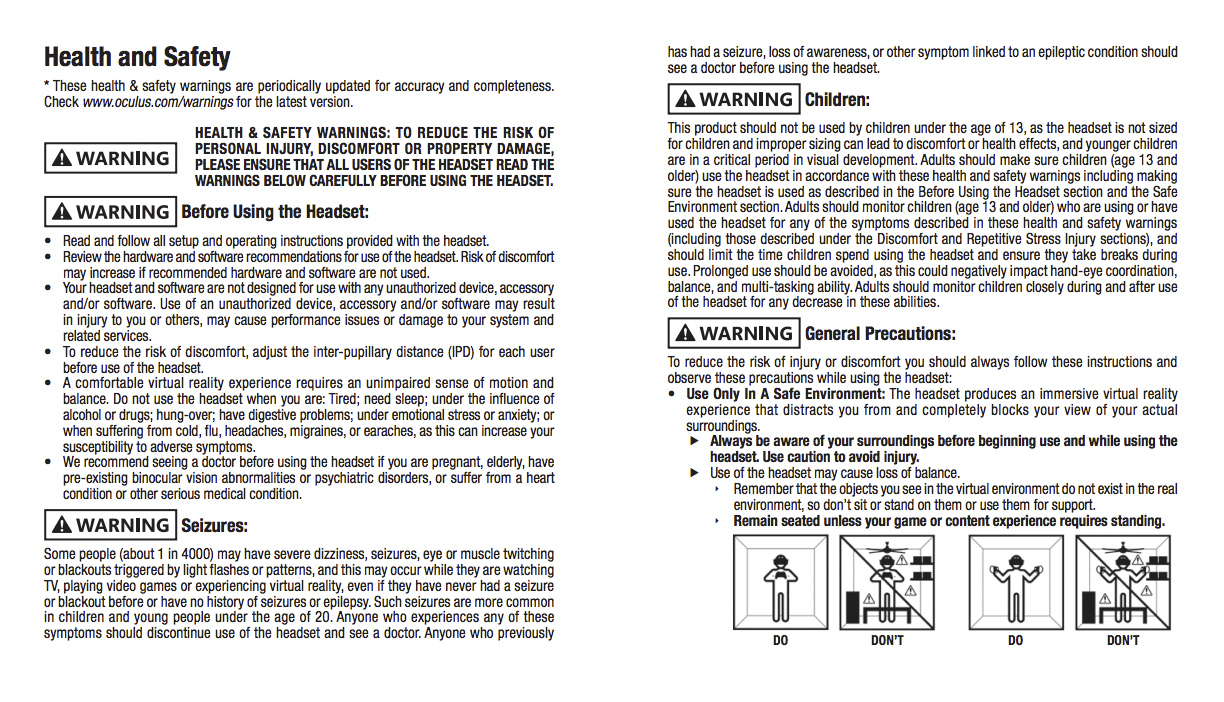
\includegraphics[scale=.45]{assets/sideeffects}  }
	\end{center}

\end{frame}

\begin{frame}
	\frametitle{Sound}
	
	Sound is a pressure wave in a material medium (air or water for example) created when an object vibrates back and forth. The frequency of the sound is dependant on the number of full oscillations that occur during one second. 
	\\~\\
	Humans can hear frequencies from roughly 20 to 22,000Hz but are most comfortable with frequencies of 2,000 - 4000Hz, Why? \pause
	\\~\\
	Most useful for speech recognition!

\end{frame}

\begin{frame}
	\frametitle{Binaural Sound}
	``Binaural recording means constructing an accurate artificial head, and placing microphones in the position of the eardrums. The resulting audio accurately records the effect of the sound travelling through the skull and ears, resulting in incredibly accurate positional sound that can be played back through any standard stereo headphones.''
	\\~\\
``Although it is a challenging technical task this can be simulated digitally, resulting in a a more immersive experience for all headphone wearing players, but of huge benefit for players with impaired vision, allowing accurate enough spatial awareness to navigate 3D environments via standard stereo headphones.'' \\~\\
	\tiny{http://gameaccessibilityguidelines.com/}
\end{frame}

\begin{frame}
	\frametitle{Two Big Ears}
	
	\begin{center}
		\href{http://www.twobigears.com/index.php}{
\includegraphics[scale=.4]{assets/twobigears} }
	\end{center}
	
\end{frame}

\begin{frame}
	\frametitle{ Head Related Transfer Functions (HRTF)}
``HRTFs work by filtering an audio signal to recreate the complex cues that help us, as humans, localise sounds. The cues are influenced by
multiple factors, including the listening environment and the shape of your body, head and ears. In reality, we
move our heads and reorient ourselves to localise sounds. We constantly try to bring sounds (or the objects that
are creating such sounds) into our line of sight to overcome the ambiguity of spatialisation.'' \\~\\

\end{frame}

\begin{frame}
	\frametitle{Balance}
	There are three systems at work to aid in balance:
	
	\begin{itemize}
		\item Vestibular System (motion, equilibrium, spatial orientation)
		\item Proprioception (position, motion, and equilibrium)
		\item Vision (sight)
	\end{itemize}
			
\end{frame}

\begin{frame}
	\frametitle{Vestibular System}
	\begin{center}
		\href{https://www.youtube.com/watch?v=P3aYqxGesqs}{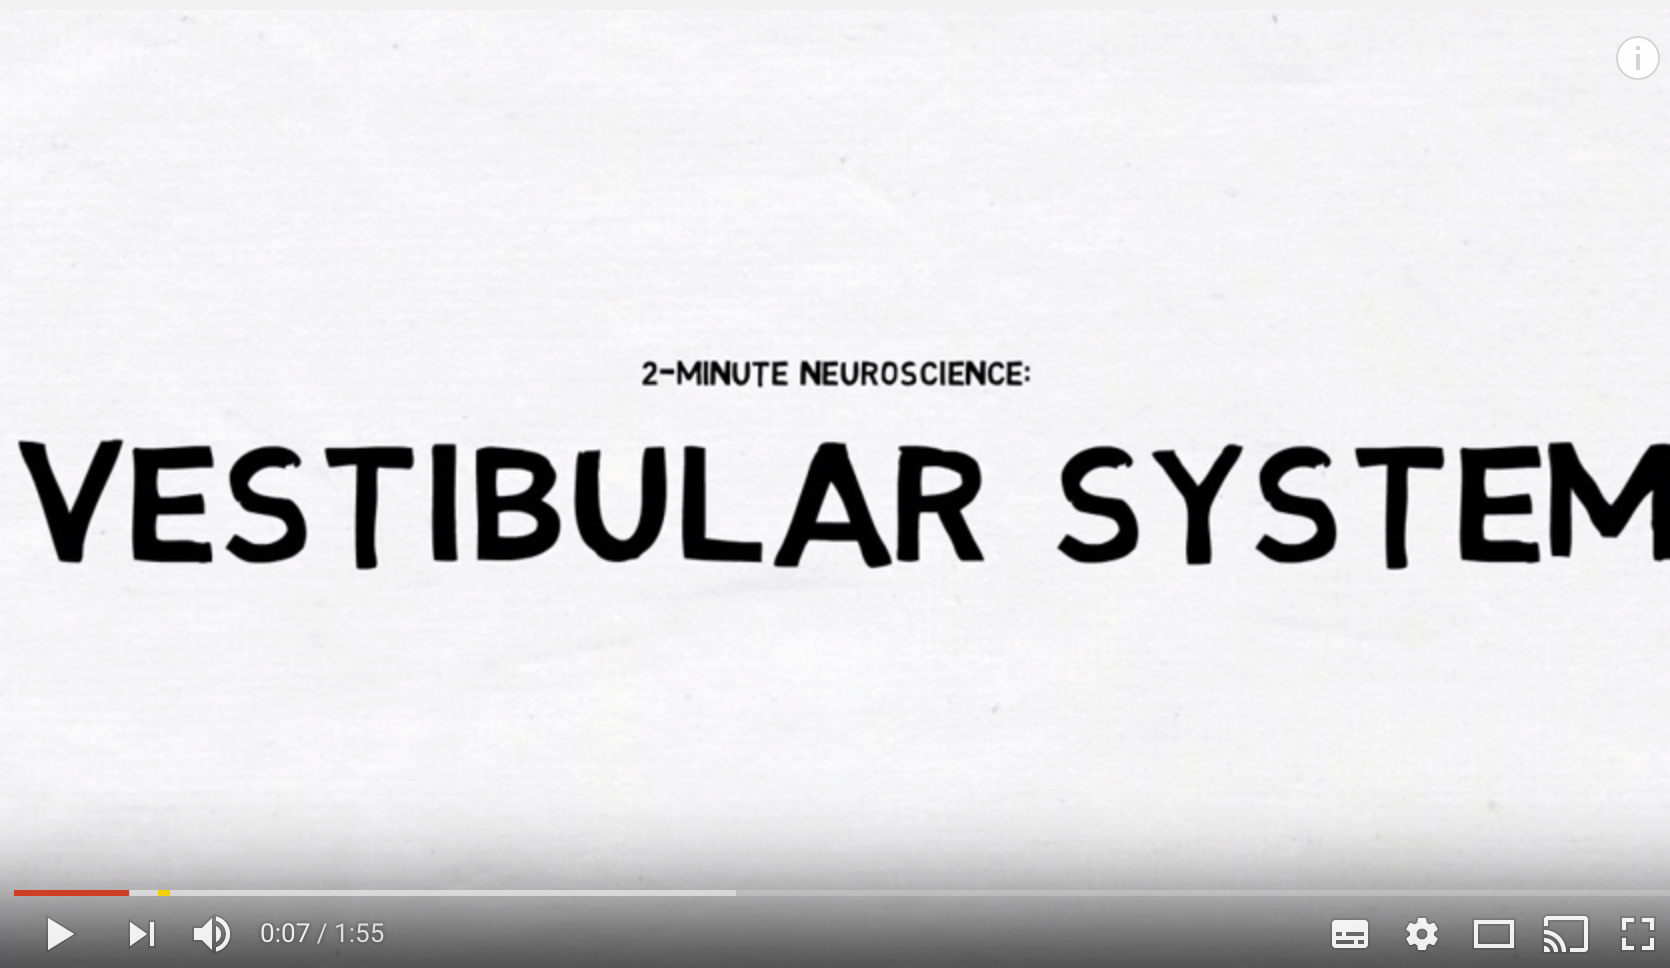
\includegraphics[scale=.3]{assets/vestibular} }
	\end{center}
\end{frame}

\begin{frame}
	Visually induced motion sickness (VIMS) is a specific type of motion sickness caused by a conflict between vision and both the proprioception and vestibular systems.  \\~\\
	
	According to \href{http://www.forbes.com/sites/kevinmurnane/2016/03/28/keeping-your-balance-with-an-oculus-rift/#36ac747823d7}{Forbes}, when a player is cycling a bike in VR, they have a tendency to lean to accommodate for corning, and as a consequence they fall off. \\~\\
	
	When tradition big screens cause VIMS the viewer can just look away but in VR this is not possible. 
	

\end{frame}

\begin{frame}
	\frametitle{Eye Tracking Demo} 
\end{frame}


\end{document}
